\chapter{Мультиплеты \texorpdfstring{\(SU(5)\)}{SU(5)}, калибровочные бозоны-лептокварки и распад протона}

\lectureoverview{Великое объединение становится конкретным, когда группа Стандартной модели вкладывается в \(SU(5)\). Чтобы увидеть, что означает это утверждение, мы сначала построим необходимую теорию представлений: определяющее представление \(N\), его сопряжённое \(\overline N\), тензорные произведения, симметричные и антисимметричные тензоры и присоединённое представление. Тогда одно семейство Стандартной модели укладывается в неожиданно экономичную комбинацию \(\overline{\mathbf 5}\oplus\mathbf{10}\). Та же симметрия, которая делает эту схему красивой, также требует цветных калибровочных бозонов, превращающих кварки в лептоны. Их обмен допускает распад протона, вынуждая масштаб объединения смещаться к \(10^{15}\)--\(10^{16}\,\mathrm{GeV}\). Бегущие калибровочные константы связи указывают на сходный масштаб, а в конце мы снова вернёмся к суперсимметрии, потому что она делает их численное совпадение существенно более точным.}

\section{Почему начинать с групповых представлений?}

Существует много предложенных теорий великого объединения. Вместо их обзора мы разберём один пример и зададим три вопроса: что заставляет его работать, каких новых частиц он требует и в чём эксперимент ставит его под угрозу. Эта группа — \(SU(5)\), а её определяющая структурная особенность состоит во вложении
\begin{equation}
SU(3)_c\times SU(2)_L\times U(1)_Y
\subset SU(5).
\label{eq:l10-sm-embedding}
\end{equation}
Здесь \(SU(3)_c\) действует на цвет, \(SU(2)_L\) — на слабый изоспин, а \(U(1)_Y\) — на гиперзаряд.

Суперсимметрия не является предпосылкой этой конструкции. Ни суперсимметрия логически не влечёт великого объединения, ни великое объединение — суперсимметрии. Их связь в этой лекции численная: когда в расчёт по группе ренормализации включается спектр суперпартнёров, три калибровочные константы связи точнее сходятся к общему значению.

Частицы, которые симметрия смешивает между собой, образуют представление группы симметрии. Поэтому классификация унифицированных мультиплетов частиц сначала требует небольшой теории представлений.

\subsection{Знакомый пример \texorpdfstring{\(SU(2)\)}{SU(2)}}

Группа \(SU(2)\), связанная с обычным моментом импульса, тесно связана с вращениями трёхмерного пространства. Точнее, \(SU(2)\) является двулистным накрытием \(SO(3)\). Её неприводимые представления помечаются величиной
\begin{equation}
j=0,\frac12,1,\frac32,\ldots,
\qquad
\dim(j)=2j+1.
\label{eq:l10-su2-spins}
\end{equation}
Поэтому скаляр является синглетом, частица со спином \(\tfrac12\) — дублетом, а частица со спином один — триплетом. Слабая группа \(SU(2)_L\) представляет собой другую физическую симметрию, хотя её абстрактная теория групп та же.

\section{Определяющее представление и его сопряжённое}

Для \(SU(N)\) определяющее представление — это пространство комплексных столбцов с \(N\) компонентами,
\begin{equation}
\psi=
\begin{pmatrix}
\psi_1\\
\psi_2\\
\vdots\\
\psi_N
\end{pmatrix},
\qquad
\psi'_i=U_i{}^j\psi_j,
\qquad
U\in SU(N).
\label{eq:l10-defining}
\end{equation}
Его называют либо определяющим представлением, либо просто \(\mathbf N\). Матрицы \(U\) имеют размер \(N\times N\), а векторное пространство, на котором они действуют, имеет размерность \(N\).

Комплексное сопряжение даёт другое \(N\)-мерное представление,
\begin{equation}
\psi_i^*\longmapsto U_i{}^{j*}\psi_j^*,
\label{eq:l10-conjugate}
\end{equation}
обозначаемое как \(\overline{\mathbf N}\). При \(N>2\) определяющее и сопряжённое представления неэквивалентны. Можно поменять местами, какое из них называть представлением частицы, а какое — представлением античастицы, но, выбрав соглашение, нужно далее его сохранять.

\begin{classroomqa}
\audiencequestion{Зависит ли \(N\) в \(SU(N)\) от того, чётно \(N\) или нечётно, и относится ли оно к матрицам? \lecturetimestamp{00:07:33}}
\lecturerresponse{Здесь нет никакого ограничения по признаку чётности--нечётности. \(N\) — это размер определяющих матриц, а также размерность их определяющего представления. И \(\mathbf N\), и \(\overline{\mathbf N}\) имеют эту размерность.}
\end{classroomqa}

Античастица античастицы есть исходная частица. Вот почему перестановка названий \(\mathbf N\) и \(\overline{\mathbf N}\) меняет соглашение, а не физику.

\section{Тензорные произведения и неприводимость}

Предположим, что один объект может находиться в \(N\) внутренних состояниях и другой объект независимо может находиться в таком же числе состояний. Игнорируя положение, импульс, спин и все квантовые числа, кроме этой метки \(SU(N)\), пара имеет
\begin{equation}
N\times N=N^2
\label{eq:l10-product-count}
\end{equation}
состояний. Если первый объект находится в состоянии \(\psi_i\), а второй — в состоянии \(\phi_j\), их произведение можно записать как
\begin{equation}
\Psi_{ij}=\psi_i\phi_j,
\qquad
\Psi'_{ij}=U_i{}^kU_j{}^\ell\Psi_{k\ell}.
\label{eq:l10-tensor-transform}
\end{equation}
Это тензорное произведение \(\mathbf N\otimes\mathbf N\).

\begin{classroomqa}
\audiencequestion{Почему ответ равен \(N^2\), а не \(N^2-1\), и не нарушает ли допущение, что обе частицы имеют одну и ту же внутреннюю метку, принцип запрета Паули? \lecturetimestamp{00:10:22}}
\lecturerresponse{Эти два места здесь различимы: один объект фиксирован в одной точке, а другой — в другой. Принцип Паули накладывает ограничения на полное квантовое состояние, включая положение. Он не устраняет ни одной из этих \(N^2\) комбинаций внутренних меток. Число \(N^2-1\) появится позже из условия бесследовости в другом произведении.}
\end{classroomqa}

\(N^2\)-мерное произведение представлений, вообще говоря, приводимо. Представление приводимо, если оно содержит собственное подпространство, которое группа переводит в себя. Такие инвариантные подпространства можно отделить и рассматривать как меньшие представления; если никакого такого собственного подпространства не существует, представление неприводимо.

\subsection{Симметричные и антисимметричные тензоры}

Всякий тензор с двумя индексами единственным образом разлагается на
\begin{align}
\Psi_{ij}
&=\Psi^{(S)}_{ij}+\Psi^{(A)}_{ij},\\
\Psi^{(S)}_{ij}
&=\frac12(\Psi_{ij}+\Psi_{ji}),\\
\Psi^{(A)}_{ij}
&=\frac12(\Psi_{ij}-\Psi_{ji}).
\label{eq:l10-sym-anti}
\end{align}
Эти две части удовлетворяют условиям
\begin{equation}
\Psi^{(S)}_{ij}=\Psi^{(S)}_{ji},
\qquad
\Psi^{(A)}_{ij}=-\Psi^{(A)}_{ji}.
\end{equation}
Уравнение~\eqref{eq:l10-tensor-transform} сохраняет каждое из этих условий, поэтому групповые преобразования никогда не смешивают симметрический и антисимметрический секторы.

\editorialnote{В лекции общий подсчёт оставлен как упражнение. Размерности симметрической и антисимметрической частей равны \(N(N+1)/2\) и \(N(N-1)/2\) соответственно, а их сумма равна \(N^2\).}

\begin{figure}[htbp]
\centering
\includegraphics[width=0.78\textwidth]{lecture_10_figure_02.png}
\lectureframe{00:17:57.500}
\caption{Завершённое разложение на доске для двух состояний со спином \(\tfrac12\): три симметричных состояния и одно антисимметричное состояние.}
\label{fig:l10-spin-decomposition}
\end{figure}

Для определяющего дублета \(SU(2)\),
\begin{equation}
\mathbf2\otimes\mathbf2=\mathbf3_S\oplus\mathbf1_A.
\label{eq:l10-two-two}
\end{equation}
Если обозначить два базисных состояния как \(u\) и \(d\), то симметрический триплет имеет вид
\begin{align}
\ket{1,1}&=\ket{uu},\\
\ket{1,0}&=\frac{1}{\sqrt2}\bigl(\ket{ud}+\ket{du}\bigr),\\
\ket{1,-1}&=\ket{dd},
\end{align}
тогда как антисимметрический синглет равен
\begin{equation}
\ket{0,0}
=\frac{1}{\sqrt2}\bigl(\ket{ud}-\ket{du}\bigr).
\end{equation}
Это знакомое сложение двух спиновых угловых моментов \(\tfrac12\): четыре исходных состояния перегруппировываются в спин один и спин ноль.

\section{Частица и античастица: присоединённое представление}

Теперь объединим определяющее представление с его сопряжённым. Произведение по-прежнему имеет \(N^2\) компонент, но преобразуется как матрица:
\begin{equation}
M_i{}^j\in\mathbf N\otimes\overline{\mathbf N},
\qquad
M\longmapsto U M U^\dagger.
\label{eq:l10-matrix-transform}
\end{equation}
В отличие от \(\mathbf N\otimes\mathbf N\), между одним фундаментальным и одним антифундаментальным индексом нет осмысленной симметрии перестановки. Естественное разложение здесь вместо этого таково:
\begin{equation}
M
=
\frac{\operatorname{tr}M}{N}\,\mathbf1_N
+
\left(M-\frac{\operatorname{tr}M}{N}\,\mathbf1_N\right).
\label{eq:l10-trace-split}
\end{equation}
Первый член является синглетом, а бесследовая часть — присоединённым представлением:
\begin{equation}
\mathbf N\otimes\overline{\mathbf N}
=\mathbf1\oplus\mathbf{Adj},
\qquad
\dim\mathbf{Adj}=N^2-1.
\label{eq:l10-adjoint}
\end{equation}

\begin{figure}[htbp]
\centering
\includegraphics[width=0.67\textwidth]{lecture_10_figure_04.png}
\lectureframe{00:23:47.500}
\caption{Вывод на доске для \(\mathbf N\otimes\overline{\mathbf N}\): его \(N^2-1\) бесследовых компонент образуют присоединённое представление.}
\label{fig:l10-adjoint}
\end{figure}

Для \(SU(3)\) это даёт знакомый октет,
\begin{equation}
\mathbf3\otimes\overline{\mathbf3}
=\mathbf8\oplus\mathbf1,
\end{equation}
и 8 глюонов преобразуются по присоединённому представлению. Для \(SU(2)\) присоединённое представление имеет размерность 3 и преобразуется как спин 1.

\section{Одно семейство Стандартной модели}

Наблюдаются три поколения, но \(SU(5)\) повторяет одно и то же построение отдельно для каждого. Это не объясняет, почему существует три копии. Поэтому мы сосредоточимся на первом поколении.

Все поля будут записаны как левые вейлевские поля. Правый фермион представляется своим левым зарядово-сопряжённым полем:
\begin{equation}
u^c_L,\qquad d^c_L,\qquad e^c_L.
\label{eq:l10-left-handed-bookkeeping}
\end{equation}
Верхний индекс \(c\) обозначает зарядовое сопряжение; например, \(d^c_L\) — это левое поле анти-d-кварка с электрическим зарядом \(+\tfrac13\).

В стандартных обозначениях \(SU(5)\) пять из пятнадцати левых полей объединяются в
\begin{equation}
\overline{\mathbf5}
=
\begin{pmatrix}
\nu_{eL}\\
e_L\\
d^c_{rL}\\
d^c_{gL}\\
d^c_{bL}
\end{pmatrix}.
\label{eq:l10-fivebar}
\end{equation}
Порядок выбран так, что сначала идёт двумерный слабый блок, а затем трёхмерный цветовой блок. Слабые преобразования смешивают первые две компоненты, цветовые преобразования смешивают последние три, а внедиагональные генераторы \(SU(5)\) соединяют эти два блока.

\editorialnote{В лекции столбец в уравнении~\eqref{eq:l10-fivebar} называется \(\mathbf5\), а позднее антисимметричный мультиплет называется \(\overline{\mathbf{10}}\). Это глобально сопряжённая конвенция. Мы используем современный стандарт \(\overline{\mathbf5}\oplus\mathbf{10}\); если сопрячь каждое представление, то обозначения лекции воспроизводятся без изменения её физики.}

Полный минимальный набор полей первого поколения имеет вид
\begin{equation}
\begin{gathered}
\underbrace{Q_L=(u_L,d_L)}_{6}
\oplus
\underbrace{L_L=(\nu_{eL},e_L)}_{2},\\
\underbrace{u^c_L}_{3}
\oplus
\underbrace{d^c_L}_{3}
\oplus
\underbrace{e^c_L}_{1},\\
6+2+3+3+1=15.
\end{gathered}
\label{eq:l10-fifteen}
\end{equation}
В минимальной Стандартной модели нет независимого \(\nu^c_L\), поэтому она не даёт перенормируемой массы нейтрино. Нейтринные осцилляции показывают, что это минимальное утверждение неполно: в природе существуют малые ненулевые массы нейтрино, и требуется расширение.

\begin{classroomqa}
\audiencequestion{Когда масса фермиона переводит левое состояние в правое, превращает ли она также частицу в её античастицу? \lecturetimestamp{00:34:00}}
\lecturerresponse{Нет. Масса электрона связывает левый электрон с правым электроном того же электрического заряда. В нотации, где все поля левые, второе поле представляется как \(e^c_L\), но четырёхкомпонентная частица остаётся электроном. Только нейтральное поле может иметь майорановскую массу, которая отождествляет частицу и античастицу.}
\end{classroomqa}

\section{Калибровочные бозоны, видимые в пятёрке}

Каждому генератору калибровочной симметрии соответствует калибровочное поле. В уравнении~\eqref{eq:l10-fivebar} уже можно распознать знакомые переходы:
\begin{itemize}
\item слабые калибровочные поля действуют между \(\nu_{eL}\) и \(e_L\);
\item глюоны действуют между тремя цветами \(d^c_L\);
\item нейтральные генераторы действуют по диагонали;
\item новые недиагональные генераторы превращают лептонную компоненту в цветную или наоборот.
\end{itemize}

Глюон можно представить как несущий цветовые квантовые числа пары кварк--антикварк. В лекции используется обычная мнемоника мировых линий: проследите вылетающий антикварк назад через вершину испускания, и он будет выглядеть как кварк, движущийся вперёд. Поэтому испущенное поле несёт квантовые числа пары кварк--антикварк. На языке представлений это в точности бесследовая часть \(\mathbf3\otimes\overline{\mathbf3}\).

Для \(SU(5)\),
\begin{equation}
\dim\mathbf{Adj}_{SU(5)}=5^2-1=24.
\end{equation}
Разложение этих калибровочных полей относительно подгруппы Стандартной модели имеет вид
\begin{equation}
\mathbf{24}
=
(\mathbf8,\mathbf1)_0
\oplus(\mathbf1,\mathbf3)_0
\oplus(\mathbf1,\mathbf1)_0
\oplus(\mathbf3,\mathbf2)_{-5/6}
\oplus(\overline{\mathbf3},\mathbf2)_{5/6},
\label{eq:l10-adjoint-sm}
\end{equation}
где упорядоченная пара обозначает \(SU(3)_c\times SU(2)_L\), а нижний индекс — гиперзаряд.

\editorialnote{Уравнение~\eqref{eq:l10-adjoint-sm} явно показывает блочную структуру, изображённую в лекции. Первые три члена содержат знакомые цветовые и электрослабые калибровочные поля. Последние два члена — это двенадцать вещественных степеней свободы, которые по принятому соглашению называют бозонами \(X\) и \(Y\).}

\begin{figure}[htbp]
\centering
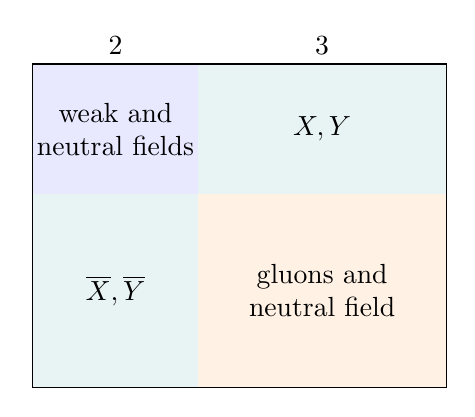
\begin{tikzpicture}[x=1.05cm,y=0.82cm]
  \draw[thick] (0,0) rectangle (5,5);
  \draw[thick] (2,0) -- (2,5);
  \draw[thick] (0,3) -- (5,3);
  \fill[blue!9] (0,3) rectangle (2,5);
  \fill[orange!10] (2,0) rectangle (5,3);
  \fill[teal!9] (2,3) rectangle (5,5);
  \fill[teal!9] (0,0) rectangle (2,3);
  \node[align=center] at (1,4) {weak and\\neutral fields};
  \node[align=center] at (3.5,1.5) {gluons and\\neutral field};
  \node[align=center] at (3.5,4) {\(X,Y\)};
  \node[align=center] at (1,1.5) {\(\overline X,\overline Y\)};
  \node[above] at (1,5) {\(2\)};
  \node[above] at (3.5,5) {\(3\)};
\end{tikzpicture}
\caption{Блочная структура \(2\oplus3\) калибровочного поля \(SU(5)\). Недиагональные блоки соединяют лептоны и цветные поля.}
\label{fig:l10-gauge-blocks}
\end{figure}

При \(Q=T_3+Y\) цветной слабый дублет в уравнении~\eqref{eq:l10-adjoint-sm} имеет заряды \(-\tfrac13\) и \(-\tfrac43\); его сопряжение имеет заряды \(+\tfrac13\) и \(+\tfrac43\). В лекции эти частицы называются \(X\) и \(Y\), но при этом явно не фиксируется, какое имя какому заряду соответствует. Переход и заряд составляют инвариантное содержание.

\begin{classroomqa}
\audiencequestion{Существуют ли три версии каждого нового калибровочного бозона \(X\) или \(Y\)? \lecturetimestamp{00:41:28}}
\lecturerresponse{Да. Переход соединяет цветную кварковую компоненту с бесцветной лептонной компонентой, поэтому обмениваемый бозон должен нести недостающий цвет. Поля \(X/Y\) образуют цветовые триплеты и могут испускать или поглощать глюоны.}
\end{classroomqa}

Цветные частицы не наблюдаются как изолированные асимптотические состояния. Новые калибровочные бозоны должны распадаться или адронизоваться в цветонейтральные комбинации, точно так же, как кварки.

\section{Почему мультиплет содержит антидаун-кварки}

Генераторы \(SU(N)\) — это бесследовые эрмитовы матрицы. Чтобы увидеть связь со словом «special», запишем бесконечно малый элемент группы в виде
\begin{equation}
U(\epsilon)=e^{i\epsilon T}.
\end{equation}
Унитарность даёт \(T^\dagger=T\), тогда как
\begin{equation}
1=\det U=e^{i\epsilon\operatorname{tr}T}
\end{equation}
для произвольного \(\epsilon\) даёт
\begin{equation}
\operatorname{tr}T=0.
\label{eq:l10-traceless-generator}
\end{equation}

Электрический заряд есть линейная комбинация генераторов. В столбце полей материи в уравнении ~\eqref{eq:l10-fivebar} он действует как
\begin{equation}
Q_{\overline5}
=
\operatorname{diag}
\left(0,-1,\frac13,\frac13,\frac13\right),
\qquad
\operatorname{tr}Q_{\overline5}=0.
\label{eq:l10-charge-fivebar}
\end{equation}
Следовательно,
\begin{equation}
0-1+3\left(\frac13\right)=0.
\end{equation}
При замене антидаун-полей на даун-поля получилось бы
\begin{equation}
0-1+3\left(-\frac13\right)=-2,
\end{equation}
что не может быть следом генератора \(SU(5)\). Поэтому это на первый взгляд странное приписывание антидаун-полей диктуется групповой структурой.

\section{Оставшиеся десять фермионов}

Остальные десять полей получаются из антисимметрического тензора с двумя индексами. В стандартном соглашении это антисимметрическая часть
\begin{equation}
\mathbf5\otimes\mathbf5
=\mathbf{15}_S\oplus\mathbf{10}_A.
\label{eq:l10-five-five}
\end{equation}
На лекции его строят, временно записывая сопряжённые квантовые числа
\begin{equation}
\chi=
\begin{pmatrix}
\nu^c\\
e^c\\
d_r\\
d_g\\
d_b
\end{pmatrix}.
\label{eq:l10-aux-five}
\end{equation}
Это лишь вспомогательный приём для тензорного произведения представлений, а не утверждение о том, что существует второй физический пятиплет составных частиц.

Пусть
\begin{equation}
\Psi^{ij}=-\Psi^{ji},
\qquad
i,j=1,\ldots,5.
\label{eq:l10-antisym-ten}
\end{equation}
Все диагональные элементы равны нулю, а нижнетреугольная часть определяется верхнетреугольной. Следовательно,
\begin{equation}
\dim\mathbf{10}
=\binom52
=\frac{5\cdot4}{2}
=10.
\label{eq:l10-ten-count}
\end{equation}

Электрический заряд элемента равен сумме зарядов строки и столбца в уравнении ~\eqref{eq:l10-aux-five}. Отсюда сразу получаются \(e^c\) в позиции weak--weak, даун- и ап-кварки в блоках weak--color, а анти-ап-поля в блоке color--color.

\begin{classroomqa}
\audiencequestion{Когда объединяются обозначения позитрона и даун-кварка, должен ли получающийся элемент быть бозоном \(X\)? \lecturetimestamp{00:53:08}}
\lecturerresponse{Нет. На этом этапе мы строим фермионное представление, а не адъюнктное представление калибровочных бозонов. Заряды складываются как \(1-\tfrac13=\tfrac23\), поэтому элемент имеет квантовые числа ап-кварка.}
\end{classroomqa}

Согласованный выбор цветовых знаков таков:
\begin{equation}
\Psi^{ij}=
\begin{pmatrix}
0 & e^c & d_r & d_g & d_b\\
-e^c & 0 & u_r & u_g & u_b\\
-d_r & -u_r & 0 & u_b^c & -u_g^c\\
-d_g & -u_g & -u_b^c & 0 & u_r^c\\
-d_b & -u_b & u_g^c & -u_r^c & 0
\end{pmatrix}.
\label{eq:l10-ten-matrix}
\end{equation}
Изменение фаз полей меняет некоторые выписанные знаки, но не представление и не состав частиц.

\begin{figure}[htbp]
\centering
\includegraphics[width=0.83\textwidth]{lecture_10_figure_05.png}
\lectureframe{00:59:17.500}
\caption{Ничем не загороженная \(2\oplus3\) антисимметрическая матрица материи после того, как на занятии были проверены её элементы и цветовые метки.}
\label{fig:l10-ten-board}
\end{figure}

\begin{classroomqa}
\audiencequestion{Должно ли десяти-мерное представление быть записано в виде матрицы, или его можно записать столбцом? \lecturetimestamp{00:56:24}}
\lecturerresponse{Возможны оба варианта. Можно перечислить десять независимых компонент в столбец, но антисимметрическая матрица \(5\times5\) показывает, как \(SU(5)\) действует на оба её индекса, и потому гораздо информативнее.}
\end{classroomqa}

\begin{classroomqa}
\audiencequestion{В блоке color--color элемент, помеченный как \(u\), на самом деле должен быть анти-ап-полем? \lecturetimestamp{00:57:51}}
\lecturerresponse{Да. Надпись на доске исправляется на \(u^c\), то есть на левое анти-ап-поле. Два базисных заряда даун-типа в сумме дают \(-\tfrac23\), что и есть электрический заряд анти-ап-кварка.}
\end{classroomqa}

\begin{classroomqa}
\audiencequestion{В нескольких элементах матрицы цветовые метки опущены. Сохраняется ли цвет по-прежнему? \lecturetimestamp{00:58:05}}
\lecturerresponse{Да. Три цветовых слота соответствуют красному, зелёному и синему. Метки опущены лишь для того, чтобы не загромождать запись.}
\end{classroomqa}

Антисимметричная пара цветовых фундаментальных представлений преобразуется как антицвет:
\begin{equation}
\wedge^2\mathbf3\simeq\overline{\mathbf3},
\qquad
(rg,rb,gb)\sim(\overline b,-\overline g,\overline r).
\label{eq:l10-anticolor}
\end{equation}
Именно поэтому три независимых элемента в блоке цвет--цвет образуют в точности цветовой триплет анти-up-кварка.

Одно поколение теперь собрано в виде
\begin{equation}
\overline{\mathbf5}\oplus\mathbf{10}.
\label{eq:l10-family}
\end{equation}
Поразительно, что \(u_L\) и \(u^c_L\) входят в один неприводимый мультиплет, тогда как \(d_L\) и \(d^c_L\), или \(e_L\) и \(e^c_L\), находятся в разных мультиплетах.

\begin{classroomqa}
\audiencequestion{Если калибровочные преобразования действуют только внутри каждого представления, как масса может связывать поля, лежащие в пятёрке с чертой и десятке? \lecturetimestamp{01:00:40}}
\lecturerresponse{Калибровочные бозоны не поворачивают одно неприводимое представление материи в другое. Поля Хиггса и юкавские связи могут соединять разные представления, образуя при этом в целом \(SU(5)\)-инвариантное взаимодействие; после того как поле Хиггса приобретает вакуумное среднее, эти взаимодействия порождают массы.}
\end{classroomqa}

\section{Калибровочные бозоны действуют как сдвиги}

После того как представление собрано, действие калибровочного бозона можно понимать как сдвиг между его элементами. Нейтральный бозон может оставлять метку неизменной, слабый бозон перемещает по слабым слотам, глюон — по цветовым слотам, а бозон \(X/Y\) — между слабыми и цветовыми слотами. У заряженных калибровочных бозонов есть античастицы, поэтому каждому сдвигу соответствует обратный процесс.

Для антисимметричного тензора бесконечно малое преобразование действует на любой из двух индексов:
\begin{equation}
\delta\Psi^{ij}
=
i\epsilon
\left(
T^i{}_k\Psi^{kj}
+
T^j{}_k\Psi^{ik}
\right).
\label{eq:l10-two-index-action}
\end{equation}
В матричной картине первый член сдвигает по вертикали, а второй — по горизонтали. Составные метки, использованные для построения тензора, служат лишь мнемоникой; уравнение~\eqref{eq:l10-two-index-action} — это точное группотеоретическое утверждение.

Слабые сдвиги переводят \(d\) в \(u\); это кварковый процесс, лежащий в основе бета-распада нейтрона. Цветовые сдвиги меняют красный, зелёный и синий, не меняя аромата. Внедиагональные сдвиги делают нечто новое:
\begin{equation}
\begin{aligned}
d^c&\longleftrightarrow e,
& d^c&\longleftrightarrow\nu,\\
d&\longleftrightarrow u^c,
& u&\longleftrightarrow e^c,
\end{aligned}
\label{eq:l10-leptoquark-shifts}
\end{equation}
при этом соответствующее поле \(X/Y\) несёт разность заряда и цвета.

\begin{classroomqa}
\audiencequestion{Что означают сдвиги между четвёртым и пятым слотами, и что насчёт сдвига из первого в четвёртый? \lecturetimestamp{01:10:36}}
\lecturerresponse{Сдвиг четвёртый--пятый меняет один цвет на другой и является глюонным переходом. Сдвиг первый--четвёртый пересекает границу между слабым и цветовым блоками и является одним из новых переходов с \(X/Y\).}
\end{classroomqa}

\begin{classroomqa}
\audiencequestion{Можно ли явно заполнить один элемент нижней половины антисимметричной матрицы? \lecturetimestamp{01:11:23}}
\lecturerresponse{Да. Каждый элемент нижнего треугольника равен отрицанию транспонированного элемента верхнего треугольника. Заполнение одного делает правило наглядным; заполнение всех не добавляет никаких новых состояний.}
\end{classroomqa}

\section{Опасное следствие: распад протона}

Бозон \(X/Y\) может связывать кварк с лептоном в одной вершине и два поля кваркового типа — в другой. При импульсах, значительно меньших его массы, интегрирование по тяжёлому бозону приводит к взаимодействию размерности шесть схематического вида
\begin{equation}
\mathcal L_{\mathrm{eff}}
\sim
\frac{g_5^2}{M_X^2}\,(qq)(q\ell)
+\text{h.c.}
\label{eq:l10-effective-proton}
\end{equation}
Оно по отдельности нарушает барионное и лептонное числа, сохраняя при этом комбинации, предписываемые объединённым калибровочным взаимодействием.

На доске прослеживается судьба одного d-кварка и одного u-кварка при обмене тяжёлой частицей. d-кварк превращается в позитрон, первый u-кварк — в анти-u-кварк, а второй остаётся спектатором:
\begin{equation}
uud
\longrightarrow
e^++u\overline u.
\label{eq:l10-quark-decay}
\end{equation}
Начальное состояние — протон. Пара \(u\overline u\) может адронизоваться в нейтральный пион, что даёт
\begin{equation}
p\longrightarrow e^++\pi^0.
\label{eq:l10-proton-pion}
\end{equation}

\begin{figure}[htbp]
\centering
\includegraphics[width=0.82\textwidth]{lecture_10_figure_06.png}
\lectureframe{01:16:02.500}
\caption{Завершённое построение на доске обмена тяжёлым бозоном внутри протона, со спектаторным u-кварком и видимым каналом с позитроном.}
\label{fig:l10-proton-board}
\end{figure}

В лекции также упоминается \(p\to e^++\gamma\), где пара кварк--антикварк аннигилирует электромагнитно. Этот канал испытывает дополнительное электромагнитное подавление по сравнению с прямой адронизацией.

Эта возможность — не факультативное украшение модели. Как только простая группа содержит генераторы, связывающие кварки и лептоны, в общем случае ожидаются процессы с нарушением барионного числа. Если бы они происходили на обычных временны́х масштабах слабого или электромагнитного взаимодействия, не смогли бы существовать ни ядра, ни водород, ни макроскопическое вещество.

\section{Почему протон живёт так долго?}

\begin{classroomqa}
\audiencequestion{Является ли константа связи, порождающая бозон \(X\), той же самой объединённой константой связи, которой описывается остальная часть группы? \lecturetimestamp{01:18:34}}
\lecturerresponse{На масштабе объединения — да. Простая калибровочная теория \(SU(5)\) имеет одну калибровочную константу связи \(g_5\). Низкоэнергетические сильная, слабая и гиперзарядовая константы связи различаются, потому что после нарушения объединённой симметрии они по-разному зависят от масштаба.}
\end{classroomqa}

Константу связи нельзя выбрать фантастически малой, не отказавшись от объединённой структуры. Имеющееся подавление даёт тяжёлый пропагатор:
\begin{equation}
\mathcal A
\sim
\frac{g_5^2}{M_X^2}.
\label{eq:l10-amplitude}
\end{equation}
При возведении амплитуды в квадрат появляется \(g_5^4/M_X^4\). Оценку скорости распада завершают размерностный анализ и матричный элемент протона:
\begin{equation}
\Gamma_p
\sim
C_{\mathrm{had}}\,
\frac{\alpha_5^2\,m_p^5}{M_X^4},
\qquad
\alpha_5=\frac{g_5^2}{4\pi},
\label{eq:l10-rate}
\end{equation}
где \(C_{\mathrm{had}}\) включает групповые множители, эффекты ренормировки и непертурбативный адронный матричный элемент.

\editorialnote{В лекции выделяется существенная зависимость \(g^4/M_X^4\) и отмечается, что множители массы протона опущены. Уравнение~\eqref{eq:l10-rate} восстанавливает требуемую массовую размерность, не претендуя на точный расчёт времени жизни.}

\begin{classroomqa}
\audiencequestion{Делает ли малый множитель \(g^4\), возможно порядка \(10^{-8}\) в грубой аудиторной оценке, время жизни уже достаточно долгим? \lecturetimestamp{01:25:13}}
\lecturerresponse{Нет. Он помогает, но разрыв между микроскопическим временем сильного взаимодействия и ограничением на время жизни протона охватывает гораздо больше порядков величины. Решающее подавление должна обеспечить четвёртая степень тяжёлой массы.}
\end{classroomqa}

Если бы все массы были порядка массы протона, естественной единицей времени было бы примерно время прохождения света через протон:
\begin{equation}
t_p\sim\frac{1\ \mathrm{fm}}{c}\sim10^{-23}\ \mathrm{s}.
\label{eq:l10-proton-time}
\end{equation}
Уже само существование первичных протонов показывает, что их время жизни превышает возраст Вселенной, но лабораторные поиски идут несравненно дальше. В лекции микроскопическая оценка сравнивается с приводившимся тогда экспериментальным пределом
\begin{equation}
\tau_p\gtrsim10^{33}\ \mathrm{yr}.
\label{eq:l10-lifetime-bound}
\end{equation}

Не нужно наблюдать один протон так долго. Если бы время жизни составляло \(10^{15}\) лет, образец из \(10^{15}\) протонов давал бы примерно одно событие в год. В более общем случае, если наблюдаются \(N_p\) протонов в течение времени \(T\), ожидаемое число распадов равно
\begin{equation}
\langle n\rangle\simeq\frac{N_pT}{\tau_p}.
\label{eq:l10-event-count}
\end{equation}
Детектор, содержащий примерно \(10^{33}\) протонов, — это большой бак, а не астрономический объект: сами эти протоны имеют массу порядка \(10^6\) килограммов. Наблюдение такого образца превращает огромное индивидуальное время жизни в измеримую частоту событий или в более сильную нижнюю границу.

Совмещение уравнения~\eqref{eq:l10-rate} с ограничением на время жизни приводит к значению массы лептокваркового калибровочного бозона порядка
\begin{equation}
M_X\sim10^{15}\text{--}10^{16}\ \mathrm{GeV},
\label{eq:l10-mx}
\end{equation}
причём \(10^{16}\,\mathrm{GeV}\) в лекции используется как легко запоминающийся безопасный масштаб. Это на несколько порядков величины ниже планковского масштаба и потому не является автоматически несовместимым с квантовой теорией поля.

\section{Нарушенная \texorpdfstring{\(SU(5)\)}{SU(5)}-симметрия и масштаб объединения}

Поля \(X/Y\) входят в один присоединённый мультиплет \(SU(5)\) вместе с калибровочными полями Стандартной модели. Точная ненарушенная калибровочная симметрия не позволила бы, чтобы одни её компоненты имели массы порядка \(10^{16}\,\mathrm{GeV}\), тогда как фотон и глюоны оставались бы безмассовыми. Следовательно, эта симметрия должна быть спонтанно нарушена.

\begin{classroomqa}
\audiencequestion{Если бы симметрия \(SU(5)\) была ненарушенной, были бы все её калибровочные бозоны безмассовыми? \lecturetimestamp{01:29:37}}
\lecturerresponse{Да, в рассматриваемой калибровочной теории. Калибровочная инвариантность запрещает явную общую массу. Механизм Хиггса может придать массы калибровочным бозонам, связанным с нарушенными генераторами, оставляя при этом калибровочные поля ненарушенной подгруппы безмассовыми.}
\end{classroomqa}

Электрослабый механизм Хиггса уже иллюстрирует эту структуру: он отличает фотон от \(W^\pm\) и \(Z\). Великое объединение требует отдельного параметра порядка на высоком масштабе, который отличает слабый \(2\)-блок от цветового \(3\)-блока и делает внедиагональные поля \(X/Y\) чрезвычайно тяжёлыми.

По сравнению с \(10^{16}\,\mathrm{GeV}\) даже масса слабого бозона порядка \(100\,\mathrm{GeV}\) пренебрежимо мала. Далеко выше тяжёлого порога всеми массами калибровочных бозонов можно пренебречь, и полная симметрия \(SU(5)\) становится хорошим приближением. В этом и состоит смысл масштаба объединения: не в том, что низкоэнергетический мир явно обладает \(SU(5)\), а в том, что при достаточно больших энергиях процессы становятся нечувствительными к массовым расщеплениям, вызванным нарушением симметрии.

\section{Бегущие константы связи}

Калибровочные константы связи логарифмически зависят от энергетического масштаба. Если определить
\begin{equation}
\alpha_i(\mu)=\frac{g_i^2(\mu)}{4\pi},
\end{equation}
то однопетлевая эволюция имеет вид
\begin{equation}
\alpha_i^{-1}(\mu)
=
\alpha_i^{-1}(\mu_0)
-\frac{b_i}{2\pi}
\ln\!\left(\frac{\mu}{\mu_0}\right).
\label{eq:l10-running}
\end{equation}
Коэффициенты \(b_i\) зависят от калибровочной группы и от каждой частицы, достаточно лёгкой, чтобы циркулировать в соответствующих квантовых петлях.

\editorialnote{Чтобы сравнивать гиперзаряд с неабелевыми константами связи внутри \(SU(5)\), величине \(g_1\) нужно придать стандартную для великого объединения нормировку. Именно отсюда берутся упомянутые в лекции численные группотеоретические множители.}

При лабораторных энергиях обратные величины трёх констант связи различны. В качественном порядке, приведённом в лекции, наибольшей является \(1/\alpha_1\), поскольку гиперзарядовое взаимодействие слабее всего; затем идёт \(1/\alpha_2\), а наименьшей является \(1/\alpha_3\), поскольку сильное взаимодействие наиболее сильно. Кривые при недоступных энергиях напрямую не измеряются. Их вычисляют из наблюдаемых низкоэнергетических значений, спектра частиц и петлевых диаграмм, определяющих бета-функции. При составе частиц Стандартной модели они становятся почти прямыми линиями, если строить их как функции \(\log\mu\).

\begin{figure}[htbp]
\centering
\includegraphics[width=0.74\textwidth]{lecture_10_figure_07.png}
\lectureframe{01:36:32.500}
\caption{График на доске, показывающий сближение обратных калибровочных констант связи вблизи \(10^{16}\,\mathrm{GeV}\). Обведённая область отмечает место их неидеального совпадения.}
\label{fig:l10-running-board}
\end{figure}

Ниже порога объединения симметрия нарушена, лёгкий спектр не заполняет полных вырожденных мультиплетов \(SU(5)\), и три коэффициента бета-функций различаются. Поэтому константы связи бегут с разными скоростями. На высоком масштабе спрашивают, достигают ли они общего значения:
\begin{equation}
\alpha_1(M_{\mathrm{GUT}})
\stackrel{?}{=}
\alpha_2(M_{\mathrm{GUT}})
\stackrel{?}{=}
\alpha_3(M_{\mathrm{GUT}}).
\label{eq:l10-unification-condition}
\end{equation}

Если учитывать только несуперсимметричный спектр Стандартной модели, эти линии сближаются в области \(10^{15}\)--\(10^{16}\,\mathrm{GeV}\), но расходятся на заметную величину; в лекции говорится, что согласие составляет примерно пятнадцать процентов. Важное совпадение состоит в том, что это также масштаб, требуемый стабильностью протона.

\section{Заключительный вопрос о нейтроне}

\begin{classroomqa}
\audiencequestion{Если бы спектаторный u-кварк в диаграмме распада протона был заменён на d-кварк, описывало бы это распад нейтрона, и играл бы роль бозон \(X\)? \lecturetimestamp{01:36:40}}
\lecturerresponse{Это определяло бы великообъединённый канал нейтрона, например \(n\to e^++\pi^-\), но это не привычный распад свободного нейтрона. Обычный бета-распад нейтрона — это \(n\to p+e^-+\overline\nu_e\), и он идёт за счёт слабого взаимодействия. Если бы порядок масс протон--нейтрон был обратным, бета-стабильность также обратилась бы, тогда как гораздо более медленный великообъединённый канал мог бы сохраниться.}
\end{classroomqa}

Это различие отделяет кинематику от нового взаимодействия. То, какой нуклон испытывает бета-распад, зависит от разности масс протон--нейтрон; нарушение барионного числа при обмене \(X/Y\) — отдельный, чрезвычайно подавленный механизм.

\section{Суперсимметрия и более широкая перспектива}

Добавление спектра суперсимметричных партнёров изменяет коэффициенты бета-функций в ~\eqref{eq:l10-running}. В изложении лекции три экстраполированные константы связи тогда сходятся с точностью примерно до одного процента. Это не доказывает ни суперсимметрию, ни великое объединение, но именно по этой эмпирической причине эти две идеи часто обсуждают вместе.

Мультиплеты вещества можно объединить ещё сильнее. При
\begin{equation}
SO(10)\supset SU(5),
\end{equation}
одно спинорное представление разлагается как
\begin{equation}
\mathbf{16}
\longrightarrow
\mathbf{10}\oplus\overline{\mathbf5}\oplus\mathbf1.
\label{eq:l10-so10}
\end{equation}
Синглет естественно отождествляется с левым антинейтрино или, эквивалентно, с зарядово-сопряжённым полем правого нейтрино. Тем самым все 16 полей расширенного семейства укладываются в один неприводимый мультиплет \(SO(10)\).

Эксперименты по поиску распада протона продолжают проверять эту идею, повышая нижнюю границу на время жизни, когда события не наблюдаются. Суперсимметричные великообъединённые модели не предсказывают одного универсального времени жизни протона: дополнительные тяжёлые поля и зависящие от суперпартнёров операторы могут в широких пределах менять доминирующий канал и скорость распада.

\editorialnote{В суперсимметрическом великом объединении обмен цветным триплетом Хиггса может порождать операторы размерности 5, нарушающие барионное число, в дополнение к обсуждавшемуся здесь оператору размерности 6 с обменом калибровочного бозона. Их коэффициенты сильно зависят от тяжёлого спектра, флейворной структуры и масс суперпартнёров, что объясняет предупреждение в лекции о том, что одна лишь суперсимметрия не фиксирует никакого единственного времени жизни.}

Непреходящий урок — это скорее напряжение, чем вердикт. Теория групп с поразительной экономией объединяет кварки и лептоны, бегущие константы связи намекают на общий высокий масштаб, а суперсимметрия делает этот численный намёк более отчётливым. Та же конструкция предсказывает и опасное превращение кварков в лептоны. Поэтому любой успешный вариант должен сохранять эту элегантность и в то же время обеспечивать стабильность протона в течение почти немыслимо долгого времени. В духе заключительных слов лекции: пусть все наши протоны остаются стабильными.
